%% =============================================================================
%%  Material suplementario del articulo (documento aparte; compilar con pdfLaTeX)
%%  Contiene: la lista literal de las 180 reglas, los seis apartados del simulador por separado,
%%  figuras y tablas adicionales. Las etiquetas del articulo principal vienen de suplemento_etiquetas.tex
%%  (se regenera con codigo/gen_suplemento_etiquetas.py despues de compilar main.tex).
%% =============================================================================
\documentclass[10pt,a4paper]{article}
\usepackage[utf8]{inputenc}
\usepackage[T1]{fontenc}
\usepackage[spanish,es-tabla,es-nodecimaldot]{babel}
\usepackage[margin=2cm]{geometry}
\usepackage{amsmath,amssymb}
\usepackage{graphicx}
\usepackage{booktabs}
\usepackage[table]{xcolor}
\usepackage{longtable}
\usepackage{array}
\usepackage{url}
\usepackage{float}
\graphicspath{{figures/}}

\renewcommand{\thetable}{S\arabic{table}}
\renewcommand{\thefigure}{S\arabic{figure}}
\newcommand{\fuente}[1]{\par\vspace{3pt}\noindent{\scriptsize\textit{Fuente:} #1\par}}
\newcommand{\qbar}{\bar{q}}

% referencias cruzadas al articulo principal (etiquetas generadas desde main.aux)
% generado por codigo/gen_suplemento_etiquetas.py a partir de main.aux; no editar a mano
\expandafter\def\csname lbl@sec:intro\endcsname{I}
\expandafter\def\csname lbl@sec:sota\endcsname{II}
\expandafter\def\csname lbl@sec:sota-aislada\endcsname{II-A}
\expandafter\def\csname lbl@sec:sota-difusa\endcsname{II-B}
\expandafter\def\csname lbl@sec:sota-semaforos\endcsname{II-C}
\expandafter\def\csname lbl@fig:taxonomia\endcsname{1}
\expandafter\def\csname lbl@fig:timeline\endcsname{2}
\expandafter\def\csname lbl@tab:difusos\endcsname{1}
\expandafter\def\csname lbl@sec:sota-rl\endcsname{II-D}
\expandafter\def\csname lbl@sec:sota-repro\endcsname{II-E}
\expandafter\def\csname lbl@sec:sota-brecha\endcsname{II-F}
\expandafter\def\csname lbl@sec:modelo\endcsname{III}
\expandafter\def\csname lbl@ap:colas\endcsname{III-A}
\expandafter\def\csname lbl@eq:colaR\endcsname{1}
\expandafter\def\csname lbl@eq:retardoR\endcsname{2}
\expandafter\def\csname lbl@eq:colaG\endcsname{3}
\expandafter\def\csname lbl@eq:retardoG\endcsname{4}
\expandafter\def\csname lbl@eq:dm\endcsname{5}
\expandafter\def\csname lbl@tab:rl\endcsname{2}
\expandafter\def\csname lbl@tab:notacion\endcsname{3}
\expandafter\def\csname lbl@ap:webster\endcsname{III-B}
\expandafter\def\csname lbl@eq:webster\endcsname{6}
\expandafter\def\csname lbl@eq:retardo-webster\endcsname{7}
\expandafter\def\csname lbl@tab:variables\endcsname{4}
\expandafter\def\csname lbl@sec:controlador\endcsname{IV}
\expandafter\def\csname lbl@ap:mtlt\endcsname{IV-B}
\expandafter\def\csname lbl@eq:lt\endcsname{8}
\expandafter\def\csname lbl@eq:mt\endcsname{9}
\expandafter\def\csname lbl@ap:inferencia\endcsname{IV-D}
\expandafter\def\csname lbl@eq:mamdani\endcsname{10}
\expandafter\def\csname lbl@fig:fuzzificacion\endcsname{3}
\expandafter\def\csname lbl@eq:premisa\endcsname{11}
\expandafter\def\csname lbl@eq:decision\endcsname{12}
\expandafter\def\csname lbl@sec:ejemplo\endcsname{IV-E}
\expandafter\def\csname lbl@tab:reglas\endcsname{5}
\expandafter\def\csname lbl@tab:tabla7\endcsname{6}
\expandafter\def\csname lbl@sec:lecturas\endcsname{IV-F}
\expandafter\def\csname lbl@eq:beta\endcsname{13}
\expandafter\def\csname lbl@sec:implementacion\endcsname{V}
\expandafter\def\csname lbl@sec:metodologia\endcsname{VI}
\expandafter\def\csname lbl@sec:protocolo\endcsname{VI-B}
\expandafter\def\csname lbl@sec:comparadores\endcsname{VI-C}
\expandafter\def\csname lbl@sec:entorno\endcsname{VI-D}
\expandafter\def\csname lbl@sec:auditoria-met\endcsname{VI-E}
\expandafter\def\csname lbl@sec:resultados\endcsname{VII}
\expandafter\def\csname lbl@fig:simulador\endcsname{4}
\expandafter\def\csname lbl@sec:webster-res\endcsname{VII-B}
\expandafter\def\csname lbl@sec:tabla8\endcsname{VII-C}
\expandafter\def\csname lbl@sec:estadistica\endcsname{VII-D}
\expandafter\def\csname lbl@sec:auditoria\endcsname{VII-E}
\expandafter\def\csname lbl@tab:tablaI\endcsname{7}
\expandafter\def\csname lbl@tab:tabla8\endcsname{8}
\expandafter\def\csname lbl@fig:incertidumbre\endcsname{5}
\expandafter\def\csname lbl@tab:auditoria\endcsname{9}
\expandafter\def\csname lbl@tab:llegadas\endcsname{10}
\expandafter\def\csname lbl@sec:reglas-disparos\endcsname{VII-G}
\expandafter\def\csname lbl@fig:disparos\endcsname{6}
\expandafter\def\csname lbl@sec:ablacion\endcsname{VII-H}
\expandafter\def\csname lbl@sec:borde\endcsname{VII-I}
\expandafter\def\csname lbl@sec:verif-formulas\endcsname{VII-J}
\expandafter\def\csname lbl@tab:disparos\endcsname{11}
\expandafter\def\csname lbl@tab:ablacion\endcsname{12}
\expandafter\def\csname lbl@sec:discusion\endcsname{VIII}
\expandafter\def\csname lbl@sec:conclusiones\endcsname{IX}
\expandafter\def\csname lbl@tab:ausente\endcsname{13}
\expandafter\def\csname lbl@app:180\endcsname{A}
\expandafter\def\csname lbl@tab:matriz180\endcsname{14}

\makeatletter
\renewcommand{\ref}[1]{\@ifundefined{lbl@#1}{??}{\csname lbl@#1\endcsname}}
\renewcommand{\eqref}[1]{(\ref{#1})}
\makeatother
% las tablas del suplemento se quedan donde se escriben (ignoran el [!t] de los archivos tabla_*.tex)
\let\origtable\table\let\endorigtable\endtable
\renewenvironment{table}[1][]{\origtable[H]}{\endorigtable}

\begin{document}
\begin{center}
{\Large\bfseries Material suplementario}\\[4pt]
{\large Réplica y validación del controlador de lógica difusa para una intersección de tráfico de Pappis y Mamdani (1977): un estudio de reproducibilidad}\\[4pt]
Raul Nolberto Quispe Saya y Kevin Luis Valero Ccacya\\
{\small Escuela Profesional de Ingeniería Electrónica, Universidad Nacional de San Agustín de Arequipa}
\end{center}

Este documento acompaña al artículo principal. Las referencias a secciones, ecuaciones y tablas del artículo principal usan su numeración (las tablas y figuras de este suplemento se numeran S1, S2, \dots). Contiene: (S1) la lista literal de las 180 reglas del espacio $T\times A\times Q$ con las 25 reglas del original resaltadas; (S2) los seis apartados del simulador por separado; (S3) figuras adicionales; y (S4) tablas adicionales.

\section{Las 180 reglas del espacio $T\times A\times Q$}
Cada regla tiene la forma «si $T=t$ y $A=mt(a)$ y $Q=lt(q)$ entonces $E=t$». Las 180 reglas son las $5\times6\times6$ combinaciones de las etiquetas de las Tablas~II a~IV del original; el original usa 25 de ellas (cinco por intervención), resaltadas en verde y marcadas con $\checkmark$; las 161 restantes se marcan con $\times$. Las 25 reglas ocupan 19 filas porque varias se repiten entre intervenciones y la regla R1 usa $Q=$ any (marcada R1*), que cubre las seis filas de $T=$ very short y $A=$ none. La matriz compacta está en el Apéndice~\ref{app:180} del artículo principal; los mismos datos están en \texttt{resultados/reglas\_180.csv}.

{\scriptsize
\setlength{\tabcolsep}{3pt}
\renewcommand{\arraystretch}{1.0}
\begin{longtable}{@{}r l ccccc c@{}}
\caption{Las 180 reglas del espacio $T\times A\times Q$ ($5\times6\times6$; cada una concluye $E=T$). Las que usa el autor están resaltadas en verde y marcadas con $\checkmark$; las demás, con $\times$. Las columnas de intervención indican con qué número de regla (R1 a R5) la usa cada intervención; R1* es la regla R1 del autor, que usa $Q=$ any (no condiciona la cola) y por eso cubre las seis reglas de su fila.}
\label{tab:180}\\
\toprule
\# & Regla & 7\,s & 17\,s & 27\,s & 37\,s & 47\,s & Usada \\
\midrule
\endfirsthead
\toprule
\# & Regla & 7\,s & 17\,s & 27\,s & 37\,s & 47\,s & Usada \\
\midrule
\endhead
\midrule
\multicolumn{8}{r}{\textit{continúa en la página siguiente}}\\
\endfoot
\bottomrule
\multicolumn{8}{@{}p{0.98\textwidth}@{}}{\vspace{2pt}\textit{Fuente:} etiquetas de $T$, $A$ y $Q$ de las Tablas~II a~IV del artículo original (p.~711), combinadas por la regla del producto ($5\times6\times6=180$); reglas resaltadas: Apéndice del artículo original (pp.~715 y~716). Código: \texttt{gen\_tabla\_180.py}; mismos datos en \texttt{resultados/reglas\_180.csv}.}\\
\endlastfoot
\rowcolor{green!14}1 & \textbf{SI} $T$ = very short \textbf{Y} $A$ = mt(none) \textbf{Y} $Q$ = lt(very small) \textbf{ENTONCES} $E$ = very short & \cellcolor{green!35}R1* & \cellcolor{green!35}R1* & \cellcolor{green!35}R1* & \cellcolor{green!35}R1* & \cellcolor{green!35}R1* & \textbf{\checkmark} \\
\rowcolor{green!14}2 & \textbf{SI} $T$ = very short \textbf{Y} $A$ = mt(none) \textbf{Y} $Q$ = lt(small) \textbf{ENTONCES} $E$ = very short & \cellcolor{green!35}R1* & \cellcolor{green!35}R1* & \cellcolor{green!35}R1* & \cellcolor{green!35}R1* & \cellcolor{green!35}R1* & \textbf{\checkmark} \\
\rowcolor{green!14}3 & \textbf{SI} $T$ = very short \textbf{Y} $A$ = mt(none) \textbf{Y} $Q$ = lt(small plus) \textbf{ENTONCES} $E$ = very short & \cellcolor{green!35}R1* & \cellcolor{green!35}R1* & \cellcolor{green!35}R1* & \cellcolor{green!35}R1* & \cellcolor{green!35}R1* & \textbf{\checkmark} \\
\rowcolor{green!14}4 & \textbf{SI} $T$ = very short \textbf{Y} $A$ = mt(none) \textbf{Y} $Q$ = lt(medium) \textbf{ENTONCES} $E$ = very short & \cellcolor{green!35}R1* & \cellcolor{green!35}R1* & \cellcolor{green!35}R1* & \cellcolor{green!35}R1* & \cellcolor{green!35}R1* & \textbf{\checkmark} \\
\rowcolor{green!14}5 & \textbf{SI} $T$ = very short \textbf{Y} $A$ = mt(none) \textbf{Y} $Q$ = lt(long) \textbf{ENTONCES} $E$ = very short & \cellcolor{green!35}R1* & \cellcolor{green!35}R1* & \cellcolor{green!35}R1* & \cellcolor{green!35}R1* & \cellcolor{green!35}R1* & \textbf{\checkmark} \\
\rowcolor{green!14}6 & \textbf{SI} $T$ = very short \textbf{Y} $A$ = mt(none) \textbf{Y} $Q$ = lt(very long) \textbf{ENTONCES} $E$ = very short & \cellcolor{green!35}R1* & \cellcolor{green!35}R1* & \cellcolor{green!35}R1* & \cellcolor{green!35}R1* & \cellcolor{green!35}R1* & \textbf{\checkmark} \\
7 & \textbf{SI} $T$ = very short \textbf{Y} $A$ = mt(a few) \textbf{Y} $Q$ = lt(very small) \textbf{ENTONCES} $E$ = very short &  &  &  &  &  & $\times$ \\
8 & \textbf{SI} $T$ = very short \textbf{Y} $A$ = mt(a few) \textbf{Y} $Q$ = lt(small) \textbf{ENTONCES} $E$ = very short &  &  &  &  &  & $\times$ \\
9 & \textbf{SI} $T$ = very short \textbf{Y} $A$ = mt(a few) \textbf{Y} $Q$ = lt(small plus) \textbf{ENTONCES} $E$ = very short &  &  &  &  &  & $\times$ \\
10 & \textbf{SI} $T$ = very short \textbf{Y} $A$ = mt(a few) \textbf{Y} $Q$ = lt(medium) \textbf{ENTONCES} $E$ = very short &  &  &  &  &  & $\times$ \\
11 & \textbf{SI} $T$ = very short \textbf{Y} $A$ = mt(a few) \textbf{Y} $Q$ = lt(long) \textbf{ENTONCES} $E$ = very short &  &  &  &  &  & $\times$ \\
12 & \textbf{SI} $T$ = very short \textbf{Y} $A$ = mt(a few) \textbf{Y} $Q$ = lt(very long) \textbf{ENTONCES} $E$ = very short &  &  &  &  &  & $\times$ \\
13 & \textbf{SI} $T$ = very short \textbf{Y} $A$ = mt(few) \textbf{Y} $Q$ = lt(very small) \textbf{ENTONCES} $E$ = very short &  &  &  &  &  & $\times$ \\
14 & \textbf{SI} $T$ = very short \textbf{Y} $A$ = mt(few) \textbf{Y} $Q$ = lt(small) \textbf{ENTONCES} $E$ = very short &  &  &  &  &  & $\times$ \\
15 & \textbf{SI} $T$ = very short \textbf{Y} $A$ = mt(few) \textbf{Y} $Q$ = lt(small plus) \textbf{ENTONCES} $E$ = very short &  &  &  &  &  & $\times$ \\
16 & \textbf{SI} $T$ = very short \textbf{Y} $A$ = mt(few) \textbf{Y} $Q$ = lt(medium) \textbf{ENTONCES} $E$ = very short &  &  &  &  &  & $\times$ \\
17 & \textbf{SI} $T$ = very short \textbf{Y} $A$ = mt(few) \textbf{Y} $Q$ = lt(long) \textbf{ENTONCES} $E$ = very short &  &  &  &  &  & $\times$ \\
18 & \textbf{SI} $T$ = very short \textbf{Y} $A$ = mt(few) \textbf{Y} $Q$ = lt(very long) \textbf{ENTONCES} $E$ = very short &  &  &  &  &  & $\times$ \\
19 & \textbf{SI} $T$ = very short \textbf{Y} $A$ = mt(medium) \textbf{Y} $Q$ = lt(very small) \textbf{ENTONCES} $E$ = very short &  &  &  &  &  & $\times$ \\
20 & \textbf{SI} $T$ = very short \textbf{Y} $A$ = mt(medium) \textbf{Y} $Q$ = lt(small) \textbf{ENTONCES} $E$ = very short &  &  &  &  &  & $\times$ \\
21 & \textbf{SI} $T$ = very short \textbf{Y} $A$ = mt(medium) \textbf{Y} $Q$ = lt(small plus) \textbf{ENTONCES} $E$ = very short &  &  &  &  &  & $\times$ \\
22 & \textbf{SI} $T$ = very short \textbf{Y} $A$ = mt(medium) \textbf{Y} $Q$ = lt(medium) \textbf{ENTONCES} $E$ = very short &  &  &  &  &  & $\times$ \\
23 & \textbf{SI} $T$ = very short \textbf{Y} $A$ = mt(medium) \textbf{Y} $Q$ = lt(long) \textbf{ENTONCES} $E$ = very short &  &  &  &  &  & $\times$ \\
24 & \textbf{SI} $T$ = very short \textbf{Y} $A$ = mt(medium) \textbf{Y} $Q$ = lt(very long) \textbf{ENTONCES} $E$ = very short &  &  &  &  &  & $\times$ \\
25 & \textbf{SI} $T$ = very short \textbf{Y} $A$ = mt(many) \textbf{Y} $Q$ = lt(very small) \textbf{ENTONCES} $E$ = very short &  &  &  &  &  & $\times$ \\
26 & \textbf{SI} $T$ = very short \textbf{Y} $A$ = mt(many) \textbf{Y} $Q$ = lt(small) \textbf{ENTONCES} $E$ = very short &  &  &  &  &  & $\times$ \\
27 & \textbf{SI} $T$ = very short \textbf{Y} $A$ = mt(many) \textbf{Y} $Q$ = lt(small plus) \textbf{ENTONCES} $E$ = very short &  &  &  &  &  & $\times$ \\
28 & \textbf{SI} $T$ = very short \textbf{Y} $A$ = mt(many) \textbf{Y} $Q$ = lt(medium) \textbf{ENTONCES} $E$ = very short &  &  &  &  &  & $\times$ \\
29 & \textbf{SI} $T$ = very short \textbf{Y} $A$ = mt(many) \textbf{Y} $Q$ = lt(long) \textbf{ENTONCES} $E$ = very short &  &  &  &  &  & $\times$ \\
30 & \textbf{SI} $T$ = very short \textbf{Y} $A$ = mt(many) \textbf{Y} $Q$ = lt(very long) \textbf{ENTONCES} $E$ = very short &  &  &  &  &  & $\times$ \\
31 & \textbf{SI} $T$ = very short \textbf{Y} $A$ = mt(too many) \textbf{Y} $Q$ = lt(very small) \textbf{ENTONCES} $E$ = very short &  &  &  &  &  & $\times$ \\
32 & \textbf{SI} $T$ = very short \textbf{Y} $A$ = mt(too many) \textbf{Y} $Q$ = lt(small) \textbf{ENTONCES} $E$ = very short &  &  &  &  &  & $\times$ \\
33 & \textbf{SI} $T$ = very short \textbf{Y} $A$ = mt(too many) \textbf{Y} $Q$ = lt(small plus) \textbf{ENTONCES} $E$ = very short &  &  &  &  &  & $\times$ \\
34 & \textbf{SI} $T$ = very short \textbf{Y} $A$ = mt(too many) \textbf{Y} $Q$ = lt(medium) \textbf{ENTONCES} $E$ = very short &  &  &  &  &  & $\times$ \\
35 & \textbf{SI} $T$ = very short \textbf{Y} $A$ = mt(too many) \textbf{Y} $Q$ = lt(long) \textbf{ENTONCES} $E$ = very short &  &  &  &  &  & $\times$ \\
36 & \textbf{SI} $T$ = very short \textbf{Y} $A$ = mt(too many) \textbf{Y} $Q$ = lt(very long) \textbf{ENTONCES} $E$ = very short &  &  &  &  &  & $\times$ \\
\midrule
37 & \textbf{SI} $T$ = short \textbf{Y} $A$ = mt(none) \textbf{Y} $Q$ = lt(very small) \textbf{ENTONCES} $E$ = short &  &  &  &  &  & $\times$ \\
38 & \textbf{SI} $T$ = short \textbf{Y} $A$ = mt(none) \textbf{Y} $Q$ = lt(small) \textbf{ENTONCES} $E$ = short &  &  &  &  &  & $\times$ \\
39 & \textbf{SI} $T$ = short \textbf{Y} $A$ = mt(none) \textbf{Y} $Q$ = lt(small plus) \textbf{ENTONCES} $E$ = short &  &  &  &  &  & $\times$ \\
40 & \textbf{SI} $T$ = short \textbf{Y} $A$ = mt(none) \textbf{Y} $Q$ = lt(medium) \textbf{ENTONCES} $E$ = short &  &  &  &  &  & $\times$ \\
41 & \textbf{SI} $T$ = short \textbf{Y} $A$ = mt(none) \textbf{Y} $Q$ = lt(long) \textbf{ENTONCES} $E$ = short &  &  &  &  &  & $\times$ \\
42 & \textbf{SI} $T$ = short \textbf{Y} $A$ = mt(none) \textbf{Y} $Q$ = lt(very long) \textbf{ENTONCES} $E$ = short &  &  &  &  &  & $\times$ \\
\rowcolor{green!14}43 & \textbf{SI} $T$ = short \textbf{Y} $A$ = mt(a few) \textbf{Y} $Q$ = lt(very small) \textbf{ENTONCES} $E$ = short & \cellcolor{green!35}R2 & \cellcolor{green!35}R2 & \cellcolor{green!35}R2 &  &  & \textbf{\checkmark} \\
44 & \textbf{SI} $T$ = short \textbf{Y} $A$ = mt(a few) \textbf{Y} $Q$ = lt(small) \textbf{ENTONCES} $E$ = short &  &  &  &  &  & $\times$ \\
\rowcolor{green!14}45 & \textbf{SI} $T$ = short \textbf{Y} $A$ = mt(a few) \textbf{Y} $Q$ = lt(small plus) \textbf{ENTONCES} $E$ = short &  &  &  & \cellcolor{green!35}R2 &  & \textbf{\checkmark} \\
46 & \textbf{SI} $T$ = short \textbf{Y} $A$ = mt(a few) \textbf{Y} $Q$ = lt(medium) \textbf{ENTONCES} $E$ = short &  &  &  &  &  & $\times$ \\
\rowcolor{green!14}47 & \textbf{SI} $T$ = short \textbf{Y} $A$ = mt(a few) \textbf{Y} $Q$ = lt(long) \textbf{ENTONCES} $E$ = short &  &  &  &  & \cellcolor{green!35}R2 & \textbf{\checkmark} \\
48 & \textbf{SI} $T$ = short \textbf{Y} $A$ = mt(a few) \textbf{Y} $Q$ = lt(very long) \textbf{ENTONCES} $E$ = short &  &  &  &  &  & $\times$ \\
49 & \textbf{SI} $T$ = short \textbf{Y} $A$ = mt(few) \textbf{Y} $Q$ = lt(very small) \textbf{ENTONCES} $E$ = short &  &  &  &  &  & $\times$ \\
50 & \textbf{SI} $T$ = short \textbf{Y} $A$ = mt(few) \textbf{Y} $Q$ = lt(small) \textbf{ENTONCES} $E$ = short &  &  &  &  &  & $\times$ \\
51 & \textbf{SI} $T$ = short \textbf{Y} $A$ = mt(few) \textbf{Y} $Q$ = lt(small plus) \textbf{ENTONCES} $E$ = short &  &  &  &  &  & $\times$ \\
52 & \textbf{SI} $T$ = short \textbf{Y} $A$ = mt(few) \textbf{Y} $Q$ = lt(medium) \textbf{ENTONCES} $E$ = short &  &  &  &  &  & $\times$ \\
53 & \textbf{SI} $T$ = short \textbf{Y} $A$ = mt(few) \textbf{Y} $Q$ = lt(long) \textbf{ENTONCES} $E$ = short &  &  &  &  &  & $\times$ \\
54 & \textbf{SI} $T$ = short \textbf{Y} $A$ = mt(few) \textbf{Y} $Q$ = lt(very long) \textbf{ENTONCES} $E$ = short &  &  &  &  &  & $\times$ \\
55 & \textbf{SI} $T$ = short \textbf{Y} $A$ = mt(medium) \textbf{Y} $Q$ = lt(very small) \textbf{ENTONCES} $E$ = short &  &  &  &  &  & $\times$ \\
56 & \textbf{SI} $T$ = short \textbf{Y} $A$ = mt(medium) \textbf{Y} $Q$ = lt(small) \textbf{ENTONCES} $E$ = short &  &  &  &  &  & $\times$ \\
57 & \textbf{SI} $T$ = short \textbf{Y} $A$ = mt(medium) \textbf{Y} $Q$ = lt(small plus) \textbf{ENTONCES} $E$ = short &  &  &  &  &  & $\times$ \\
58 & \textbf{SI} $T$ = short \textbf{Y} $A$ = mt(medium) \textbf{Y} $Q$ = lt(medium) \textbf{ENTONCES} $E$ = short &  &  &  &  &  & $\times$ \\
59 & \textbf{SI} $T$ = short \textbf{Y} $A$ = mt(medium) \textbf{Y} $Q$ = lt(long) \textbf{ENTONCES} $E$ = short &  &  &  &  &  & $\times$ \\
60 & \textbf{SI} $T$ = short \textbf{Y} $A$ = mt(medium) \textbf{Y} $Q$ = lt(very long) \textbf{ENTONCES} $E$ = short &  &  &  &  &  & $\times$ \\
61 & \textbf{SI} $T$ = short \textbf{Y} $A$ = mt(many) \textbf{Y} $Q$ = lt(very small) \textbf{ENTONCES} $E$ = short &  &  &  &  &  & $\times$ \\
62 & \textbf{SI} $T$ = short \textbf{Y} $A$ = mt(many) \textbf{Y} $Q$ = lt(small) \textbf{ENTONCES} $E$ = short &  &  &  &  &  & $\times$ \\
63 & \textbf{SI} $T$ = short \textbf{Y} $A$ = mt(many) \textbf{Y} $Q$ = lt(small plus) \textbf{ENTONCES} $E$ = short &  &  &  &  &  & $\times$ \\
64 & \textbf{SI} $T$ = short \textbf{Y} $A$ = mt(many) \textbf{Y} $Q$ = lt(medium) \textbf{ENTONCES} $E$ = short &  &  &  &  &  & $\times$ \\
65 & \textbf{SI} $T$ = short \textbf{Y} $A$ = mt(many) \textbf{Y} $Q$ = lt(long) \textbf{ENTONCES} $E$ = short &  &  &  &  &  & $\times$ \\
66 & \textbf{SI} $T$ = short \textbf{Y} $A$ = mt(many) \textbf{Y} $Q$ = lt(very long) \textbf{ENTONCES} $E$ = short &  &  &  &  &  & $\times$ \\
67 & \textbf{SI} $T$ = short \textbf{Y} $A$ = mt(too many) \textbf{Y} $Q$ = lt(very small) \textbf{ENTONCES} $E$ = short &  &  &  &  &  & $\times$ \\
68 & \textbf{SI} $T$ = short \textbf{Y} $A$ = mt(too many) \textbf{Y} $Q$ = lt(small) \textbf{ENTONCES} $E$ = short &  &  &  &  &  & $\times$ \\
69 & \textbf{SI} $T$ = short \textbf{Y} $A$ = mt(too many) \textbf{Y} $Q$ = lt(small plus) \textbf{ENTONCES} $E$ = short &  &  &  &  &  & $\times$ \\
70 & \textbf{SI} $T$ = short \textbf{Y} $A$ = mt(too many) \textbf{Y} $Q$ = lt(medium) \textbf{ENTONCES} $E$ = short &  &  &  &  &  & $\times$ \\
71 & \textbf{SI} $T$ = short \textbf{Y} $A$ = mt(too many) \textbf{Y} $Q$ = lt(long) \textbf{ENTONCES} $E$ = short &  &  &  &  &  & $\times$ \\
72 & \textbf{SI} $T$ = short \textbf{Y} $A$ = mt(too many) \textbf{Y} $Q$ = lt(very long) \textbf{ENTONCES} $E$ = short &  &  &  &  &  & $\times$ \\
\midrule
73 & \textbf{SI} $T$ = medium \textbf{Y} $A$ = mt(none) \textbf{Y} $Q$ = lt(very small) \textbf{ENTONCES} $E$ = medium &  &  &  &  &  & $\times$ \\
74 & \textbf{SI} $T$ = medium \textbf{Y} $A$ = mt(none) \textbf{Y} $Q$ = lt(small) \textbf{ENTONCES} $E$ = medium &  &  &  &  &  & $\times$ \\
75 & \textbf{SI} $T$ = medium \textbf{Y} $A$ = mt(none) \textbf{Y} $Q$ = lt(small plus) \textbf{ENTONCES} $E$ = medium &  &  &  &  &  & $\times$ \\
76 & \textbf{SI} $T$ = medium \textbf{Y} $A$ = mt(none) \textbf{Y} $Q$ = lt(medium) \textbf{ENTONCES} $E$ = medium &  &  &  &  &  & $\times$ \\
77 & \textbf{SI} $T$ = medium \textbf{Y} $A$ = mt(none) \textbf{Y} $Q$ = lt(long) \textbf{ENTONCES} $E$ = medium &  &  &  &  &  & $\times$ \\
78 & \textbf{SI} $T$ = medium \textbf{Y} $A$ = mt(none) \textbf{Y} $Q$ = lt(very long) \textbf{ENTONCES} $E$ = medium &  &  &  &  &  & $\times$ \\
79 & \textbf{SI} $T$ = medium \textbf{Y} $A$ = mt(a few) \textbf{Y} $Q$ = lt(very small) \textbf{ENTONCES} $E$ = medium &  &  &  &  &  & $\times$ \\
80 & \textbf{SI} $T$ = medium \textbf{Y} $A$ = mt(a few) \textbf{Y} $Q$ = lt(small) \textbf{ENTONCES} $E$ = medium &  &  &  &  &  & $\times$ \\
81 & \textbf{SI} $T$ = medium \textbf{Y} $A$ = mt(a few) \textbf{Y} $Q$ = lt(small plus) \textbf{ENTONCES} $E$ = medium &  &  &  &  &  & $\times$ \\
82 & \textbf{SI} $T$ = medium \textbf{Y} $A$ = mt(a few) \textbf{Y} $Q$ = lt(medium) \textbf{ENTONCES} $E$ = medium &  &  &  &  &  & $\times$ \\
83 & \textbf{SI} $T$ = medium \textbf{Y} $A$ = mt(a few) \textbf{Y} $Q$ = lt(long) \textbf{ENTONCES} $E$ = medium &  &  &  &  &  & $\times$ \\
84 & \textbf{SI} $T$ = medium \textbf{Y} $A$ = mt(a few) \textbf{Y} $Q$ = lt(very long) \textbf{ENTONCES} $E$ = medium &  &  &  &  &  & $\times$ \\
\rowcolor{green!14}85 & \textbf{SI} $T$ = medium \textbf{Y} $A$ = mt(few) \textbf{Y} $Q$ = lt(very small) \textbf{ENTONCES} $E$ = medium & \cellcolor{green!35}R3 & \cellcolor{green!35}R3 & \cellcolor{green!35}R3 &  &  & \textbf{\checkmark} \\
86 & \textbf{SI} $T$ = medium \textbf{Y} $A$ = mt(few) \textbf{Y} $Q$ = lt(small) \textbf{ENTONCES} $E$ = medium &  &  &  &  &  & $\times$ \\
87 & \textbf{SI} $T$ = medium \textbf{Y} $A$ = mt(few) \textbf{Y} $Q$ = lt(small plus) \textbf{ENTONCES} $E$ = medium &  &  &  &  &  & $\times$ \\
88 & \textbf{SI} $T$ = medium \textbf{Y} $A$ = mt(few) \textbf{Y} $Q$ = lt(medium) \textbf{ENTONCES} $E$ = medium &  &  &  &  &  & $\times$ \\
89 & \textbf{SI} $T$ = medium \textbf{Y} $A$ = mt(few) \textbf{Y} $Q$ = lt(long) \textbf{ENTONCES} $E$ = medium &  &  &  &  &  & $\times$ \\
90 & \textbf{SI} $T$ = medium \textbf{Y} $A$ = mt(few) \textbf{Y} $Q$ = lt(very long) \textbf{ENTONCES} $E$ = medium &  &  &  &  &  & $\times$ \\
91 & \textbf{SI} $T$ = medium \textbf{Y} $A$ = mt(medium) \textbf{Y} $Q$ = lt(very small) \textbf{ENTONCES} $E$ = medium &  &  &  &  &  & $\times$ \\
92 & \textbf{SI} $T$ = medium \textbf{Y} $A$ = mt(medium) \textbf{Y} $Q$ = lt(small) \textbf{ENTONCES} $E$ = medium &  &  &  &  &  & $\times$ \\
\rowcolor{green!14}93 & \textbf{SI} $T$ = medium \textbf{Y} $A$ = mt(medium) \textbf{Y} $Q$ = lt(small plus) \textbf{ENTONCES} $E$ = medium &  &  &  & \cellcolor{green!35}R3 &  & \textbf{\checkmark} \\
94 & \textbf{SI} $T$ = medium \textbf{Y} $A$ = mt(medium) \textbf{Y} $Q$ = lt(medium) \textbf{ENTONCES} $E$ = medium &  &  &  &  &  & $\times$ \\
\rowcolor{green!14}95 & \textbf{SI} $T$ = medium \textbf{Y} $A$ = mt(medium) \textbf{Y} $Q$ = lt(long) \textbf{ENTONCES} $E$ = medium &  &  &  &  & \cellcolor{green!35}R3 & \textbf{\checkmark} \\
96 & \textbf{SI} $T$ = medium \textbf{Y} $A$ = mt(medium) \textbf{Y} $Q$ = lt(very long) \textbf{ENTONCES} $E$ = medium &  &  &  &  &  & $\times$ \\
97 & \textbf{SI} $T$ = medium \textbf{Y} $A$ = mt(many) \textbf{Y} $Q$ = lt(very small) \textbf{ENTONCES} $E$ = medium &  &  &  &  &  & $\times$ \\
98 & \textbf{SI} $T$ = medium \textbf{Y} $A$ = mt(many) \textbf{Y} $Q$ = lt(small) \textbf{ENTONCES} $E$ = medium &  &  &  &  &  & $\times$ \\
99 & \textbf{SI} $T$ = medium \textbf{Y} $A$ = mt(many) \textbf{Y} $Q$ = lt(small plus) \textbf{ENTONCES} $E$ = medium &  &  &  &  &  & $\times$ \\
100 & \textbf{SI} $T$ = medium \textbf{Y} $A$ = mt(many) \textbf{Y} $Q$ = lt(medium) \textbf{ENTONCES} $E$ = medium &  &  &  &  &  & $\times$ \\
101 & \textbf{SI} $T$ = medium \textbf{Y} $A$ = mt(many) \textbf{Y} $Q$ = lt(long) \textbf{ENTONCES} $E$ = medium &  &  &  &  &  & $\times$ \\
102 & \textbf{SI} $T$ = medium \textbf{Y} $A$ = mt(many) \textbf{Y} $Q$ = lt(very long) \textbf{ENTONCES} $E$ = medium &  &  &  &  &  & $\times$ \\
103 & \textbf{SI} $T$ = medium \textbf{Y} $A$ = mt(too many) \textbf{Y} $Q$ = lt(very small) \textbf{ENTONCES} $E$ = medium &  &  &  &  &  & $\times$ \\
104 & \textbf{SI} $T$ = medium \textbf{Y} $A$ = mt(too many) \textbf{Y} $Q$ = lt(small) \textbf{ENTONCES} $E$ = medium &  &  &  &  &  & $\times$ \\
105 & \textbf{SI} $T$ = medium \textbf{Y} $A$ = mt(too many) \textbf{Y} $Q$ = lt(small plus) \textbf{ENTONCES} $E$ = medium &  &  &  &  &  & $\times$ \\
106 & \textbf{SI} $T$ = medium \textbf{Y} $A$ = mt(too many) \textbf{Y} $Q$ = lt(medium) \textbf{ENTONCES} $E$ = medium &  &  &  &  &  & $\times$ \\
107 & \textbf{SI} $T$ = medium \textbf{Y} $A$ = mt(too many) \textbf{Y} $Q$ = lt(long) \textbf{ENTONCES} $E$ = medium &  &  &  &  &  & $\times$ \\
108 & \textbf{SI} $T$ = medium \textbf{Y} $A$ = mt(too many) \textbf{Y} $Q$ = lt(very long) \textbf{ENTONCES} $E$ = medium &  &  &  &  &  & $\times$ \\
\midrule
109 & \textbf{SI} $T$ = long \textbf{Y} $A$ = mt(none) \textbf{Y} $Q$ = lt(very small) \textbf{ENTONCES} $E$ = long &  &  &  &  &  & $\times$ \\
110 & \textbf{SI} $T$ = long \textbf{Y} $A$ = mt(none) \textbf{Y} $Q$ = lt(small) \textbf{ENTONCES} $E$ = long &  &  &  &  &  & $\times$ \\
111 & \textbf{SI} $T$ = long \textbf{Y} $A$ = mt(none) \textbf{Y} $Q$ = lt(small plus) \textbf{ENTONCES} $E$ = long &  &  &  &  &  & $\times$ \\
112 & \textbf{SI} $T$ = long \textbf{Y} $A$ = mt(none) \textbf{Y} $Q$ = lt(medium) \textbf{ENTONCES} $E$ = long &  &  &  &  &  & $\times$ \\
113 & \textbf{SI} $T$ = long \textbf{Y} $A$ = mt(none) \textbf{Y} $Q$ = lt(long) \textbf{ENTONCES} $E$ = long &  &  &  &  &  & $\times$ \\
114 & \textbf{SI} $T$ = long \textbf{Y} $A$ = mt(none) \textbf{Y} $Q$ = lt(very long) \textbf{ENTONCES} $E$ = long &  &  &  &  &  & $\times$ \\
115 & \textbf{SI} $T$ = long \textbf{Y} $A$ = mt(a few) \textbf{Y} $Q$ = lt(very small) \textbf{ENTONCES} $E$ = long &  &  &  &  &  & $\times$ \\
116 & \textbf{SI} $T$ = long \textbf{Y} $A$ = mt(a few) \textbf{Y} $Q$ = lt(small) \textbf{ENTONCES} $E$ = long &  &  &  &  &  & $\times$ \\
117 & \textbf{SI} $T$ = long \textbf{Y} $A$ = mt(a few) \textbf{Y} $Q$ = lt(small plus) \textbf{ENTONCES} $E$ = long &  &  &  &  &  & $\times$ \\
118 & \textbf{SI} $T$ = long \textbf{Y} $A$ = mt(a few) \textbf{Y} $Q$ = lt(medium) \textbf{ENTONCES} $E$ = long &  &  &  &  &  & $\times$ \\
119 & \textbf{SI} $T$ = long \textbf{Y} $A$ = mt(a few) \textbf{Y} $Q$ = lt(long) \textbf{ENTONCES} $E$ = long &  &  &  &  &  & $\times$ \\
120 & \textbf{SI} $T$ = long \textbf{Y} $A$ = mt(a few) \textbf{Y} $Q$ = lt(very long) \textbf{ENTONCES} $E$ = long &  &  &  &  &  & $\times$ \\
121 & \textbf{SI} $T$ = long \textbf{Y} $A$ = mt(few) \textbf{Y} $Q$ = lt(very small) \textbf{ENTONCES} $E$ = long &  &  &  &  &  & $\times$ \\
122 & \textbf{SI} $T$ = long \textbf{Y} $A$ = mt(few) \textbf{Y} $Q$ = lt(small) \textbf{ENTONCES} $E$ = long &  &  &  &  &  & $\times$ \\
123 & \textbf{SI} $T$ = long \textbf{Y} $A$ = mt(few) \textbf{Y} $Q$ = lt(small plus) \textbf{ENTONCES} $E$ = long &  &  &  &  &  & $\times$ \\
124 & \textbf{SI} $T$ = long \textbf{Y} $A$ = mt(few) \textbf{Y} $Q$ = lt(medium) \textbf{ENTONCES} $E$ = long &  &  &  &  &  & $\times$ \\
125 & \textbf{SI} $T$ = long \textbf{Y} $A$ = mt(few) \textbf{Y} $Q$ = lt(long) \textbf{ENTONCES} $E$ = long &  &  &  &  &  & $\times$ \\
126 & \textbf{SI} $T$ = long \textbf{Y} $A$ = mt(few) \textbf{Y} $Q$ = lt(very long) \textbf{ENTONCES} $E$ = long &  &  &  &  &  & $\times$ \\
\rowcolor{green!14}127 & \textbf{SI} $T$ = long \textbf{Y} $A$ = mt(medium) \textbf{Y} $Q$ = lt(very small) \textbf{ENTONCES} $E$ = long & \cellcolor{green!35}R4 & \cellcolor{green!35}R4 & \cellcolor{green!35}R4 &  &  & \textbf{\checkmark} \\
128 & \textbf{SI} $T$ = long \textbf{Y} $A$ = mt(medium) \textbf{Y} $Q$ = lt(small) \textbf{ENTONCES} $E$ = long &  &  &  &  &  & $\times$ \\
129 & \textbf{SI} $T$ = long \textbf{Y} $A$ = mt(medium) \textbf{Y} $Q$ = lt(small plus) \textbf{ENTONCES} $E$ = long &  &  &  &  &  & $\times$ \\
130 & \textbf{SI} $T$ = long \textbf{Y} $A$ = mt(medium) \textbf{Y} $Q$ = lt(medium) \textbf{ENTONCES} $E$ = long &  &  &  &  &  & $\times$ \\
131 & \textbf{SI} $T$ = long \textbf{Y} $A$ = mt(medium) \textbf{Y} $Q$ = lt(long) \textbf{ENTONCES} $E$ = long &  &  &  &  &  & $\times$ \\
132 & \textbf{SI} $T$ = long \textbf{Y} $A$ = mt(medium) \textbf{Y} $Q$ = lt(very long) \textbf{ENTONCES} $E$ = long &  &  &  &  &  & $\times$ \\
133 & \textbf{SI} $T$ = long \textbf{Y} $A$ = mt(many) \textbf{Y} $Q$ = lt(very small) \textbf{ENTONCES} $E$ = long &  &  &  &  &  & $\times$ \\
134 & \textbf{SI} $T$ = long \textbf{Y} $A$ = mt(many) \textbf{Y} $Q$ = lt(small) \textbf{ENTONCES} $E$ = long &  &  &  &  &  & $\times$ \\
135 & \textbf{SI} $T$ = long \textbf{Y} $A$ = mt(many) \textbf{Y} $Q$ = lt(small plus) \textbf{ENTONCES} $E$ = long &  &  &  &  &  & $\times$ \\
\rowcolor{green!14}136 & \textbf{SI} $T$ = long \textbf{Y} $A$ = mt(many) \textbf{Y} $Q$ = lt(medium) \textbf{ENTONCES} $E$ = long &  &  &  & \cellcolor{green!35}R4 &  & \textbf{\checkmark} \\
137 & \textbf{SI} $T$ = long \textbf{Y} $A$ = mt(many) \textbf{Y} $Q$ = lt(long) \textbf{ENTONCES} $E$ = long &  &  &  &  &  & $\times$ \\
138 & \textbf{SI} $T$ = long \textbf{Y} $A$ = mt(many) \textbf{Y} $Q$ = lt(very long) \textbf{ENTONCES} $E$ = long &  &  &  &  &  & $\times$ \\
139 & \textbf{SI} $T$ = long \textbf{Y} $A$ = mt(too many) \textbf{Y} $Q$ = lt(very small) \textbf{ENTONCES} $E$ = long &  &  &  &  &  & $\times$ \\
140 & \textbf{SI} $T$ = long \textbf{Y} $A$ = mt(too many) \textbf{Y} $Q$ = lt(small) \textbf{ENTONCES} $E$ = long &  &  &  &  &  & $\times$ \\
141 & \textbf{SI} $T$ = long \textbf{Y} $A$ = mt(too many) \textbf{Y} $Q$ = lt(small plus) \textbf{ENTONCES} $E$ = long &  &  &  &  &  & $\times$ \\
142 & \textbf{SI} $T$ = long \textbf{Y} $A$ = mt(too many) \textbf{Y} $Q$ = lt(medium) \textbf{ENTONCES} $E$ = long &  &  &  &  &  & $\times$ \\
143 & \textbf{SI} $T$ = long \textbf{Y} $A$ = mt(too many) \textbf{Y} $Q$ = lt(long) \textbf{ENTONCES} $E$ = long &  &  &  &  &  & $\times$ \\
\rowcolor{green!14}144 & \textbf{SI} $T$ = long \textbf{Y} $A$ = mt(too many) \textbf{Y} $Q$ = lt(very long) \textbf{ENTONCES} $E$ = long &  &  &  &  & \cellcolor{green!35}R4 & \textbf{\checkmark} \\
\midrule
145 & \textbf{SI} $T$ = very long \textbf{Y} $A$ = mt(none) \textbf{Y} $Q$ = lt(very small) \textbf{ENTONCES} $E$ = very long &  &  &  &  &  & $\times$ \\
146 & \textbf{SI} $T$ = very long \textbf{Y} $A$ = mt(none) \textbf{Y} $Q$ = lt(small) \textbf{ENTONCES} $E$ = very long &  &  &  &  &  & $\times$ \\
147 & \textbf{SI} $T$ = very long \textbf{Y} $A$ = mt(none) \textbf{Y} $Q$ = lt(small plus) \textbf{ENTONCES} $E$ = very long &  &  &  &  &  & $\times$ \\
148 & \textbf{SI} $T$ = very long \textbf{Y} $A$ = mt(none) \textbf{Y} $Q$ = lt(medium) \textbf{ENTONCES} $E$ = very long &  &  &  &  &  & $\times$ \\
149 & \textbf{SI} $T$ = very long \textbf{Y} $A$ = mt(none) \textbf{Y} $Q$ = lt(long) \textbf{ENTONCES} $E$ = very long &  &  &  &  &  & $\times$ \\
150 & \textbf{SI} $T$ = very long \textbf{Y} $A$ = mt(none) \textbf{Y} $Q$ = lt(very long) \textbf{ENTONCES} $E$ = very long &  &  &  &  &  & $\times$ \\
151 & \textbf{SI} $T$ = very long \textbf{Y} $A$ = mt(a few) \textbf{Y} $Q$ = lt(very small) \textbf{ENTONCES} $E$ = very long &  &  &  &  &  & $\times$ \\
152 & \textbf{SI} $T$ = very long \textbf{Y} $A$ = mt(a few) \textbf{Y} $Q$ = lt(small) \textbf{ENTONCES} $E$ = very long &  &  &  &  &  & $\times$ \\
153 & \textbf{SI} $T$ = very long \textbf{Y} $A$ = mt(a few) \textbf{Y} $Q$ = lt(small plus) \textbf{ENTONCES} $E$ = very long &  &  &  &  &  & $\times$ \\
154 & \textbf{SI} $T$ = very long \textbf{Y} $A$ = mt(a few) \textbf{Y} $Q$ = lt(medium) \textbf{ENTONCES} $E$ = very long &  &  &  &  &  & $\times$ \\
155 & \textbf{SI} $T$ = very long \textbf{Y} $A$ = mt(a few) \textbf{Y} $Q$ = lt(long) \textbf{ENTONCES} $E$ = very long &  &  &  &  &  & $\times$ \\
156 & \textbf{SI} $T$ = very long \textbf{Y} $A$ = mt(a few) \textbf{Y} $Q$ = lt(very long) \textbf{ENTONCES} $E$ = very long &  &  &  &  &  & $\times$ \\
157 & \textbf{SI} $T$ = very long \textbf{Y} $A$ = mt(few) \textbf{Y} $Q$ = lt(very small) \textbf{ENTONCES} $E$ = very long &  &  &  &  &  & $\times$ \\
158 & \textbf{SI} $T$ = very long \textbf{Y} $A$ = mt(few) \textbf{Y} $Q$ = lt(small) \textbf{ENTONCES} $E$ = very long &  &  &  &  &  & $\times$ \\
159 & \textbf{SI} $T$ = very long \textbf{Y} $A$ = mt(few) \textbf{Y} $Q$ = lt(small plus) \textbf{ENTONCES} $E$ = very long &  &  &  &  &  & $\times$ \\
160 & \textbf{SI} $T$ = very long \textbf{Y} $A$ = mt(few) \textbf{Y} $Q$ = lt(medium) \textbf{ENTONCES} $E$ = very long &  &  &  &  &  & $\times$ \\
161 & \textbf{SI} $T$ = very long \textbf{Y} $A$ = mt(few) \textbf{Y} $Q$ = lt(long) \textbf{ENTONCES} $E$ = very long &  &  &  &  &  & $\times$ \\
162 & \textbf{SI} $T$ = very long \textbf{Y} $A$ = mt(few) \textbf{Y} $Q$ = lt(very long) \textbf{ENTONCES} $E$ = very long &  &  &  &  &  & $\times$ \\
163 & \textbf{SI} $T$ = very long \textbf{Y} $A$ = mt(medium) \textbf{Y} $Q$ = lt(very small) \textbf{ENTONCES} $E$ = very long &  &  &  &  &  & $\times$ \\
164 & \textbf{SI} $T$ = very long \textbf{Y} $A$ = mt(medium) \textbf{Y} $Q$ = lt(small) \textbf{ENTONCES} $E$ = very long &  &  &  &  &  & $\times$ \\
165 & \textbf{SI} $T$ = very long \textbf{Y} $A$ = mt(medium) \textbf{Y} $Q$ = lt(small plus) \textbf{ENTONCES} $E$ = very long &  &  &  &  &  & $\times$ \\
166 & \textbf{SI} $T$ = very long \textbf{Y} $A$ = mt(medium) \textbf{Y} $Q$ = lt(medium) \textbf{ENTONCES} $E$ = very long &  &  &  &  &  & $\times$ \\
167 & \textbf{SI} $T$ = very long \textbf{Y} $A$ = mt(medium) \textbf{Y} $Q$ = lt(long) \textbf{ENTONCES} $E$ = very long &  &  &  &  &  & $\times$ \\
168 & \textbf{SI} $T$ = very long \textbf{Y} $A$ = mt(medium) \textbf{Y} $Q$ = lt(very long) \textbf{ENTONCES} $E$ = very long &  &  &  &  &  & $\times$ \\
\rowcolor{green!14}169 & \textbf{SI} $T$ = very long \textbf{Y} $A$ = mt(many) \textbf{Y} $Q$ = lt(very small) \textbf{ENTONCES} $E$ = very long & \cellcolor{green!35}R5 &  &  &  &  & \textbf{\checkmark} \\
\rowcolor{green!14}170 & \textbf{SI} $T$ = very long \textbf{Y} $A$ = mt(many) \textbf{Y} $Q$ = lt(small) \textbf{ENTONCES} $E$ = very long &  & \cellcolor{green!35}R5 & \cellcolor{green!35}R5 &  &  & \textbf{\checkmark} \\
171 & \textbf{SI} $T$ = very long \textbf{Y} $A$ = mt(many) \textbf{Y} $Q$ = lt(small plus) \textbf{ENTONCES} $E$ = very long &  &  &  &  &  & $\times$ \\
172 & \textbf{SI} $T$ = very long \textbf{Y} $A$ = mt(many) \textbf{Y} $Q$ = lt(medium) \textbf{ENTONCES} $E$ = very long &  &  &  &  &  & $\times$ \\
173 & \textbf{SI} $T$ = very long \textbf{Y} $A$ = mt(many) \textbf{Y} $Q$ = lt(long) \textbf{ENTONCES} $E$ = very long &  &  &  &  &  & $\times$ \\
174 & \textbf{SI} $T$ = very long \textbf{Y} $A$ = mt(many) \textbf{Y} $Q$ = lt(very long) \textbf{ENTONCES} $E$ = very long &  &  &  &  &  & $\times$ \\
175 & \textbf{SI} $T$ = very long \textbf{Y} $A$ = mt(too many) \textbf{Y} $Q$ = lt(very small) \textbf{ENTONCES} $E$ = very long &  &  &  &  &  & $\times$ \\
176 & \textbf{SI} $T$ = very long \textbf{Y} $A$ = mt(too many) \textbf{Y} $Q$ = lt(small) \textbf{ENTONCES} $E$ = very long &  &  &  &  &  & $\times$ \\
177 & \textbf{SI} $T$ = very long \textbf{Y} $A$ = mt(too many) \textbf{Y} $Q$ = lt(small plus) \textbf{ENTONCES} $E$ = very long &  &  &  &  &  & $\times$ \\
178 & \textbf{SI} $T$ = very long \textbf{Y} $A$ = mt(too many) \textbf{Y} $Q$ = lt(medium) \textbf{ENTONCES} $E$ = very long &  &  &  &  &  & $\times$ \\
\rowcolor{green!14}179 & \textbf{SI} $T$ = very long \textbf{Y} $A$ = mt(too many) \textbf{Y} $Q$ = lt(long) \textbf{ENTONCES} $E$ = very long &  &  &  & \cellcolor{green!35}R5 &  & \textbf{\checkmark} \\
\rowcolor{green!14}180 & \textbf{SI} $T$ = very long \textbf{Y} $A$ = mt(too many) \textbf{Y} $Q$ = lt(very long) \textbf{ENTONCES} $E$ = very long &  &  &  &  & \cellcolor{green!35}R5 & \textbf{\checkmark} \\
\end{longtable}
}


\clearpage
\section{Los seis apartados del simulador}
Las figuras siguientes muestran, ampliados, los seis apartados de la ventana del simulador (Fig.~\ref{fig:simulador} del artículo principal). Corresponden al escenario 720/2160\,veh/h, lectura calibrada y semilla 1, en $t=118$\,s (un instante posterior en 1\,s al de la Fig.~\ref{fig:simulador} del artículo principal), cuando el controlador decide extender 4\,s el verde del brazo E-W en la intervención de 47\,s, por la regla R2.

\begin{figure}[!h]
\centering
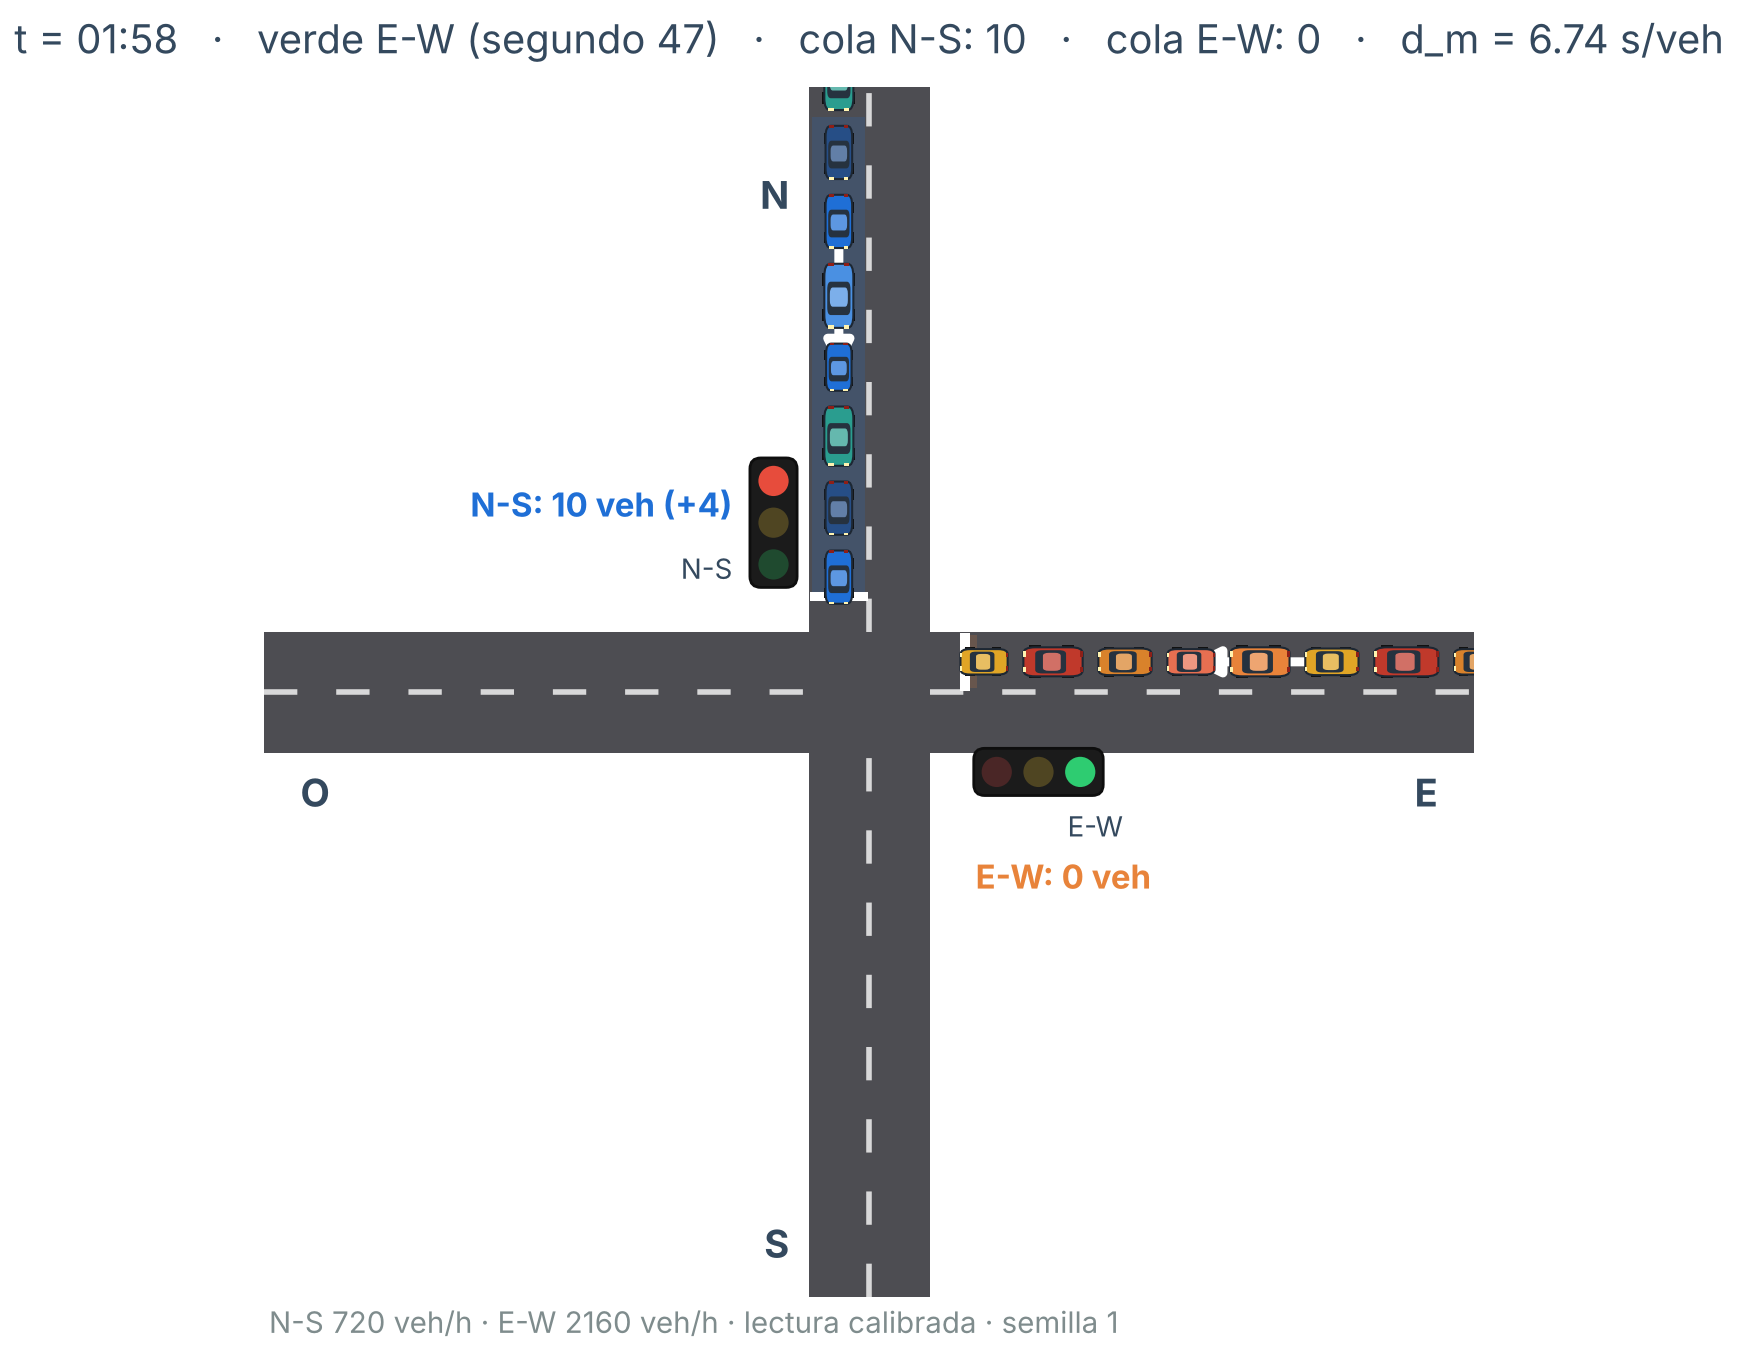
\includegraphics[width=0.62\textwidth]{fig_sim_calle.png}
\caption{(a) La calle: cruce con vehículos en movimiento (azul: N-S; naranja: E-W), semáforos de tres luces, colas y encabezado con el tiempo y $d_m$.}
\end{figure}

\begin{figure}[!h]
\centering
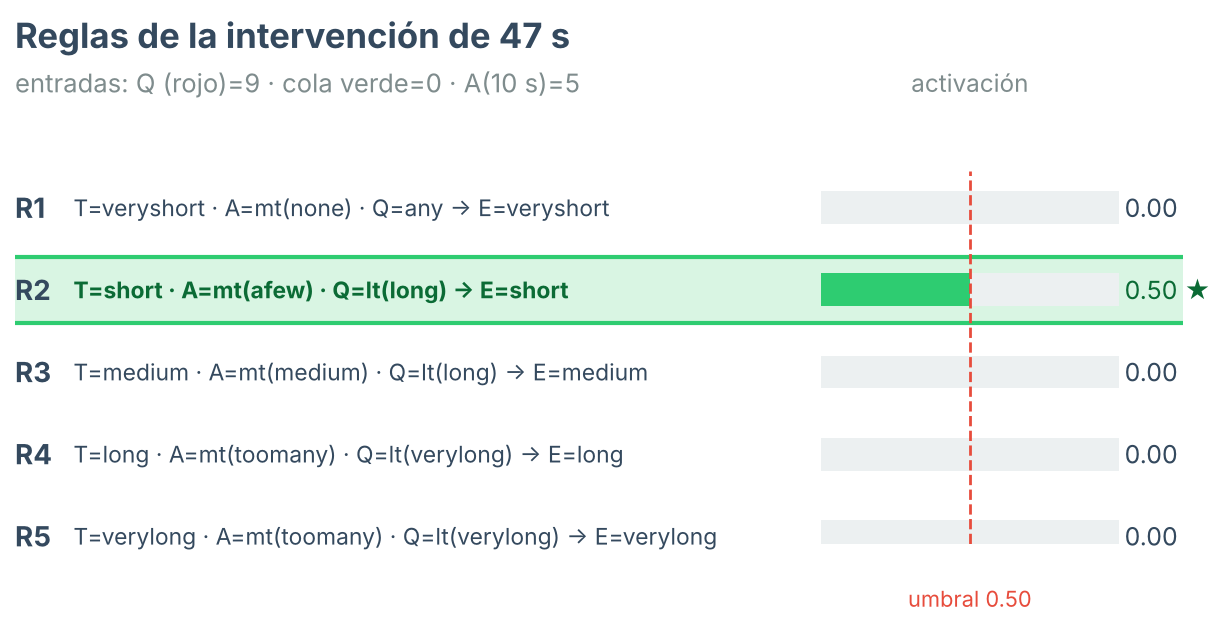
\includegraphics[width=0.8\textwidth]{fig_sim_reglas.png}
\caption{(b) Panel de reglas de la intervención de 47\,s: entradas de la decisión, activación de cada regla y regla que dispara ($\star$, R2).}
\end{figure}

\begin{figure}[!h]
\centering
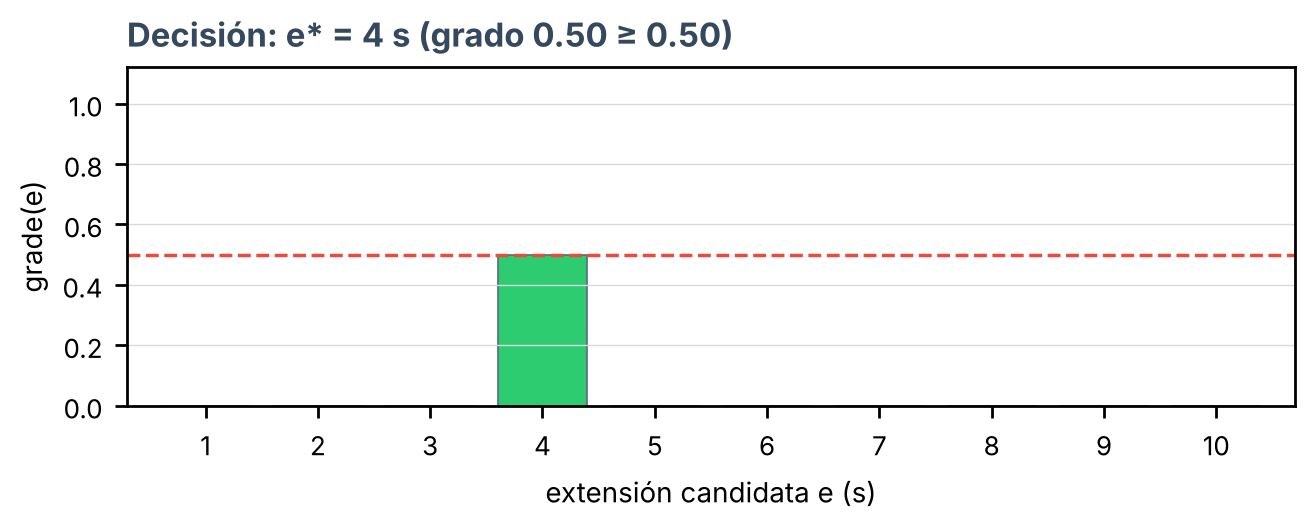
\includegraphics[width=0.75\textwidth]{fig_sim_decision.png}
\caption{(c) Vector de grados $\gamma(e)$ de las extensiones candidatas, umbral 0.5 y extensión elegida ($e^*=4$\,s, grado 0.50).}
\end{figure}

\begin{figure}[!h]
\centering
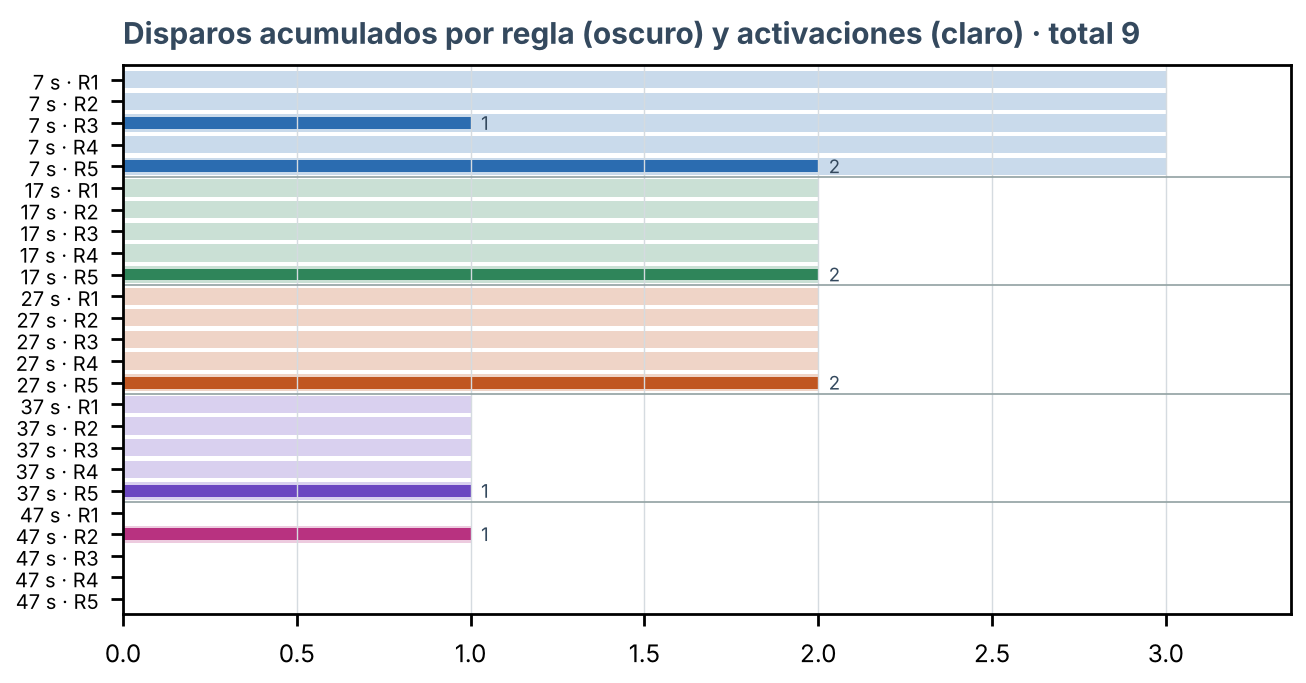
\includegraphics[width=0.75\textwidth]{fig_sim_disparos.png}
\caption{(d) Disparos acumulados (barra oscura) y activaciones (barra clara) de las 25 reglas, agrupadas por intervención, hasta $t=118$\,s.}
\end{figure}

\begin{figure}[!h]
\centering
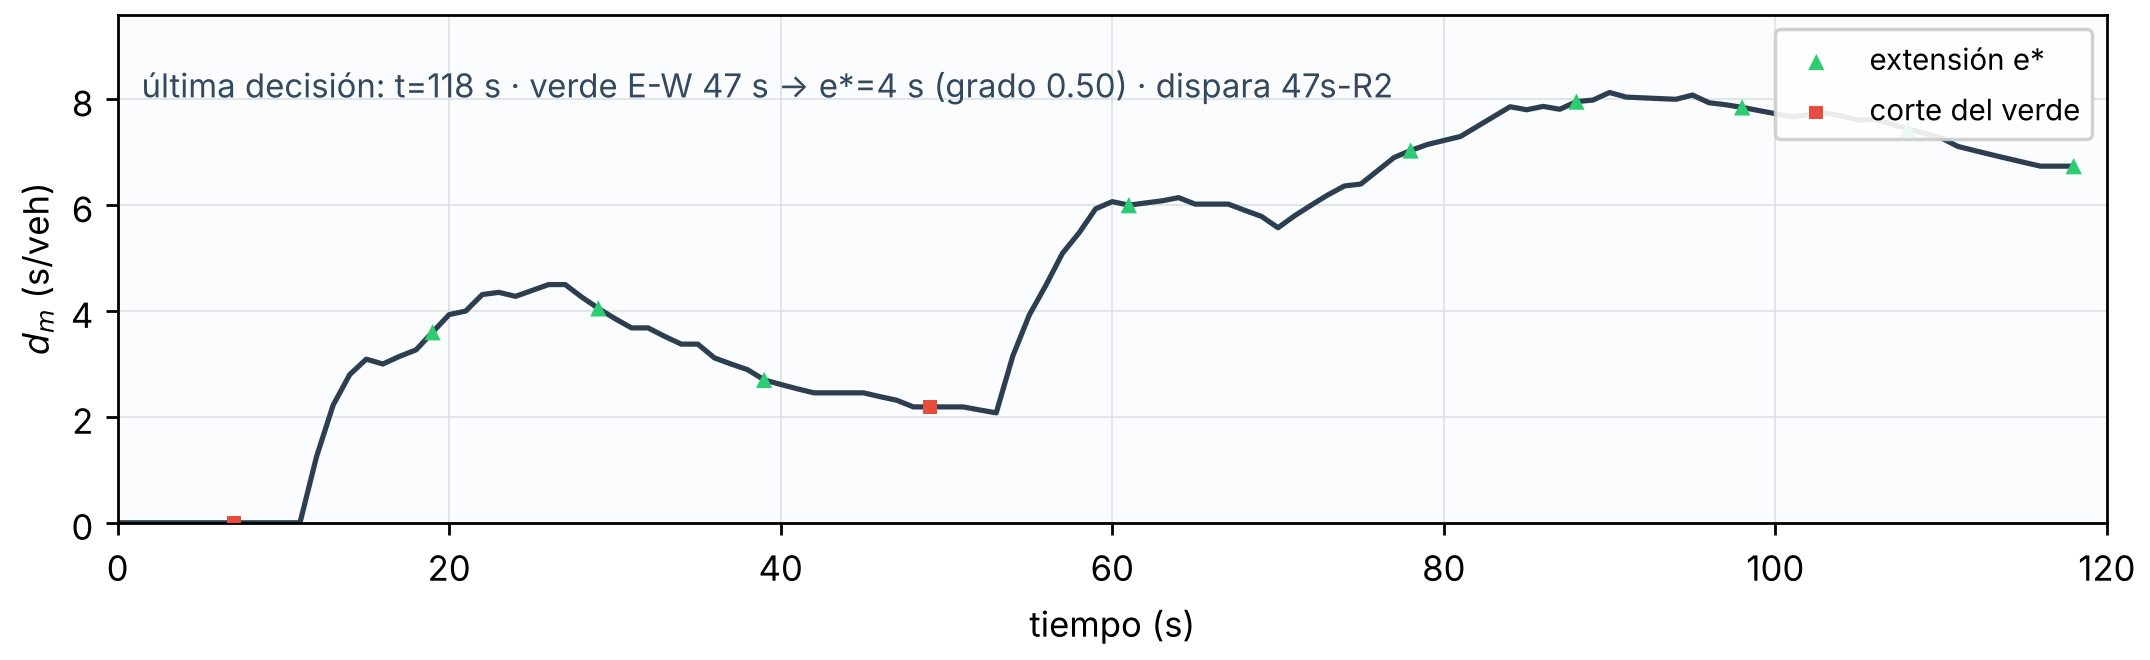
\includegraphics[width=0.95\textwidth]{fig_sim_traza.png}
\caption{(e) Traza del retardo medio $d_m$ en el tiempo. Los triángulos verdes marcan las extensiones del verde y los cuadrados rojos, los cortes.}
\end{figure}

\begin{figure}[!h]
\centering
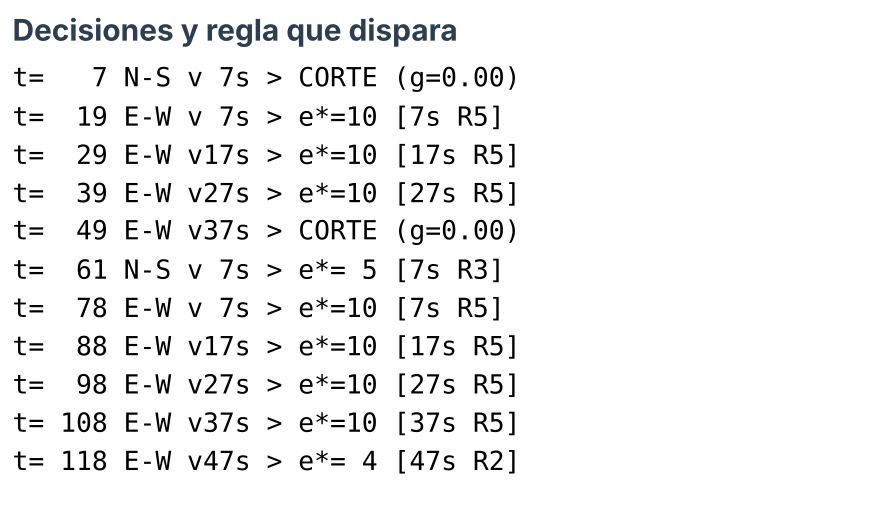
\includegraphics[width=0.55\textwidth]{fig_sim_registro.png}
\caption{(f) Registro de decisiones: tiempo, brazo en verde, segundo de verde, extensión elegida y regla que dispara.}
\end{figure}

\clearpage
\section{Figuras adicionales}

\begin{figure}[!h]
\centering
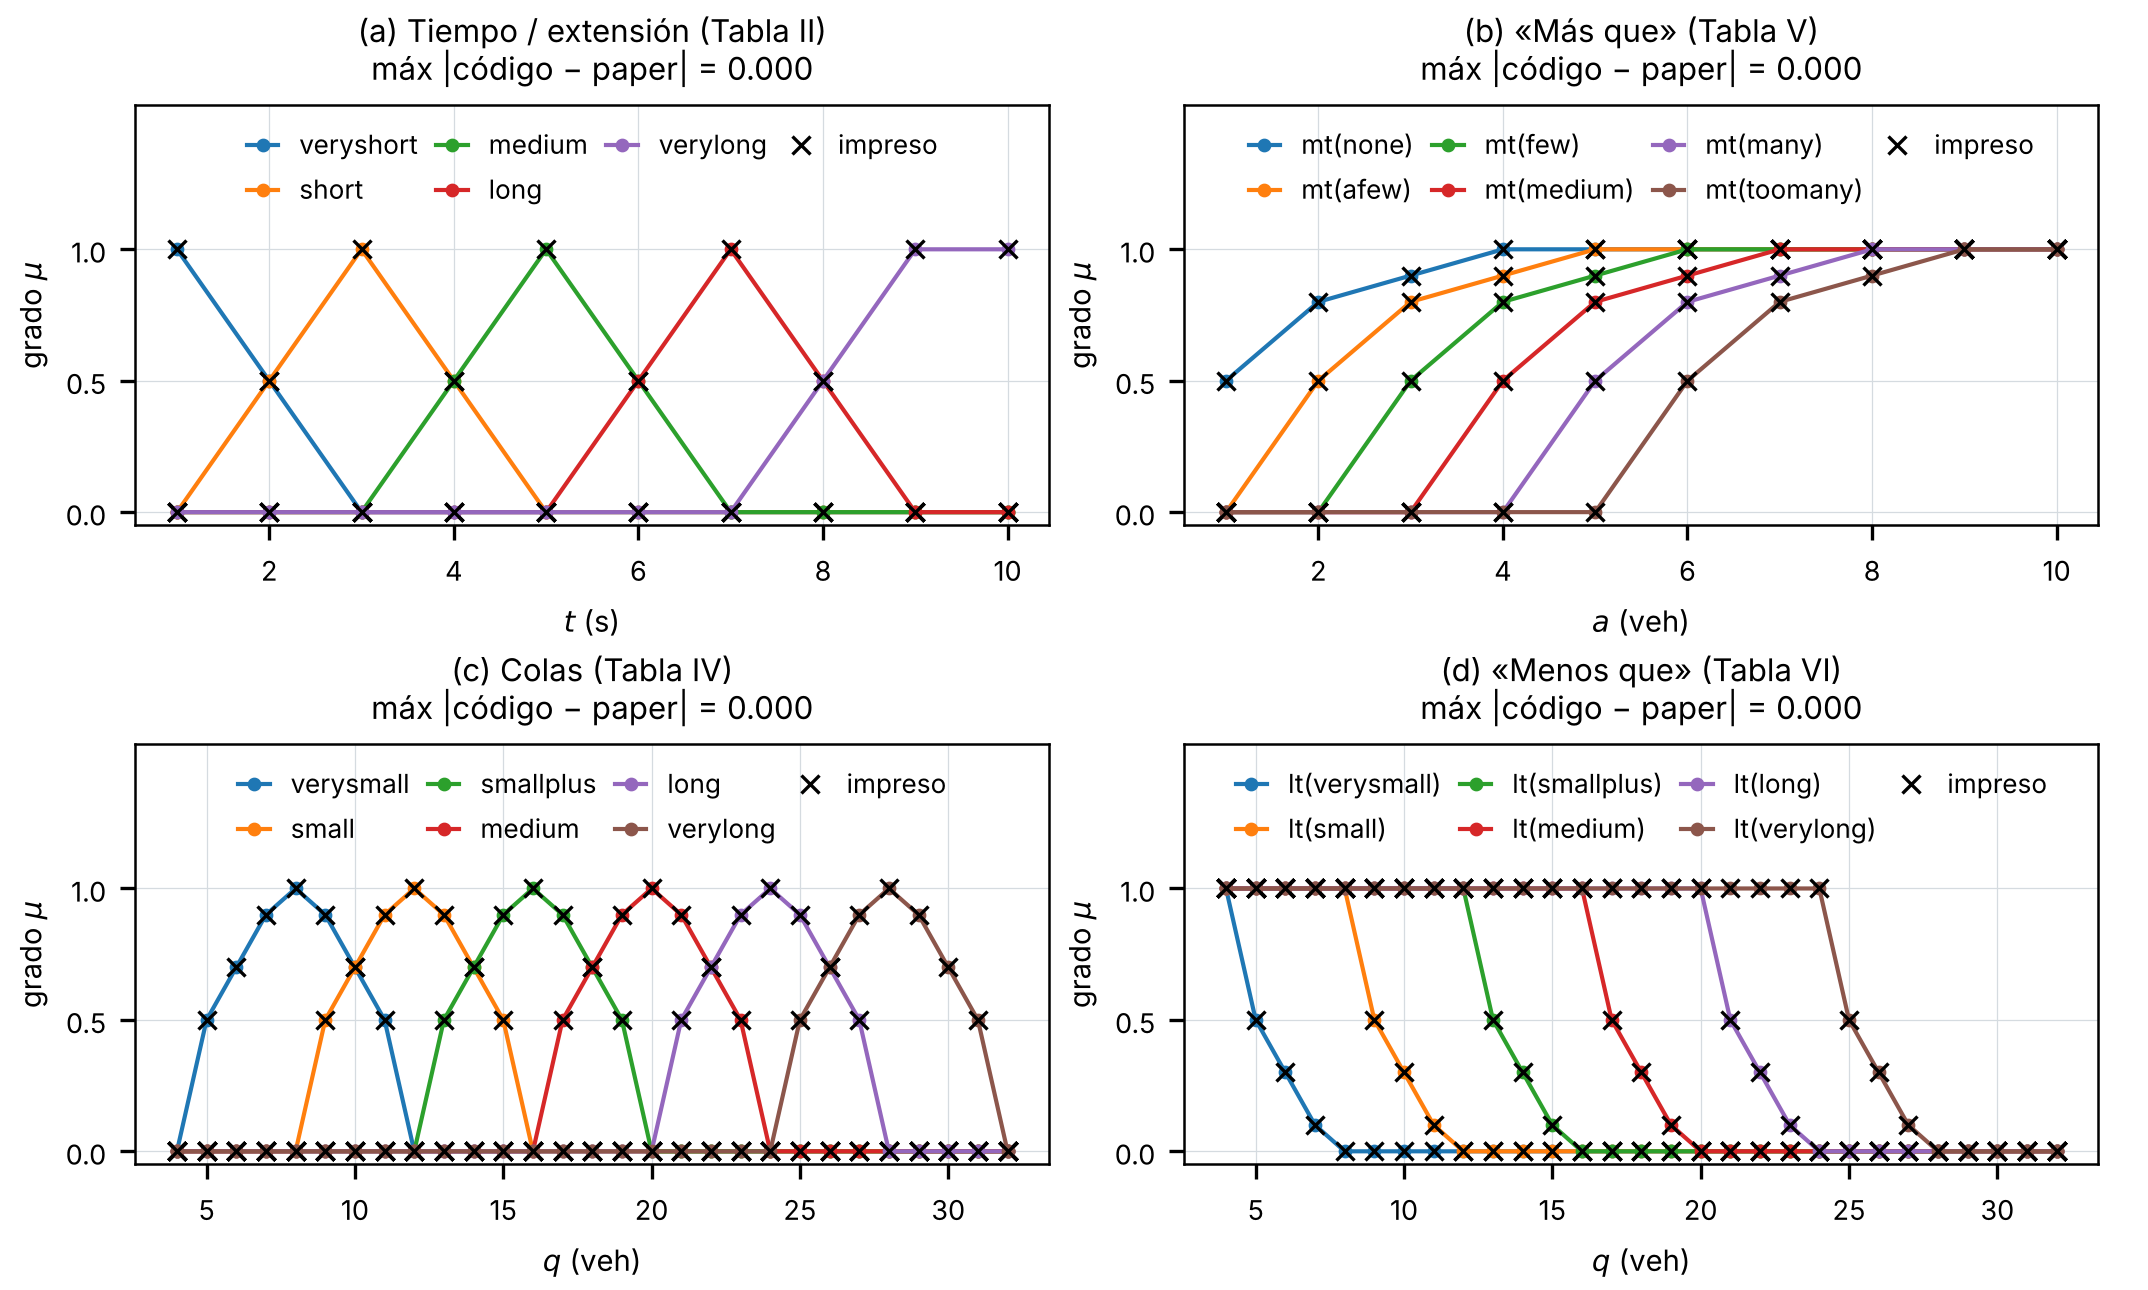
\includegraphics[width=\textwidth]{fig_validacion_curvas.png}
\caption{Validación de la fuzzificación: curvas del código (líneas) y valores impresos en el artículo original ($\times$) para las Tablas~II, IV, V y~VI del original. La diferencia máxima es 0.000 en los cuatro paneles.}
\end{figure}

\begin{figure}[!h]
\centering
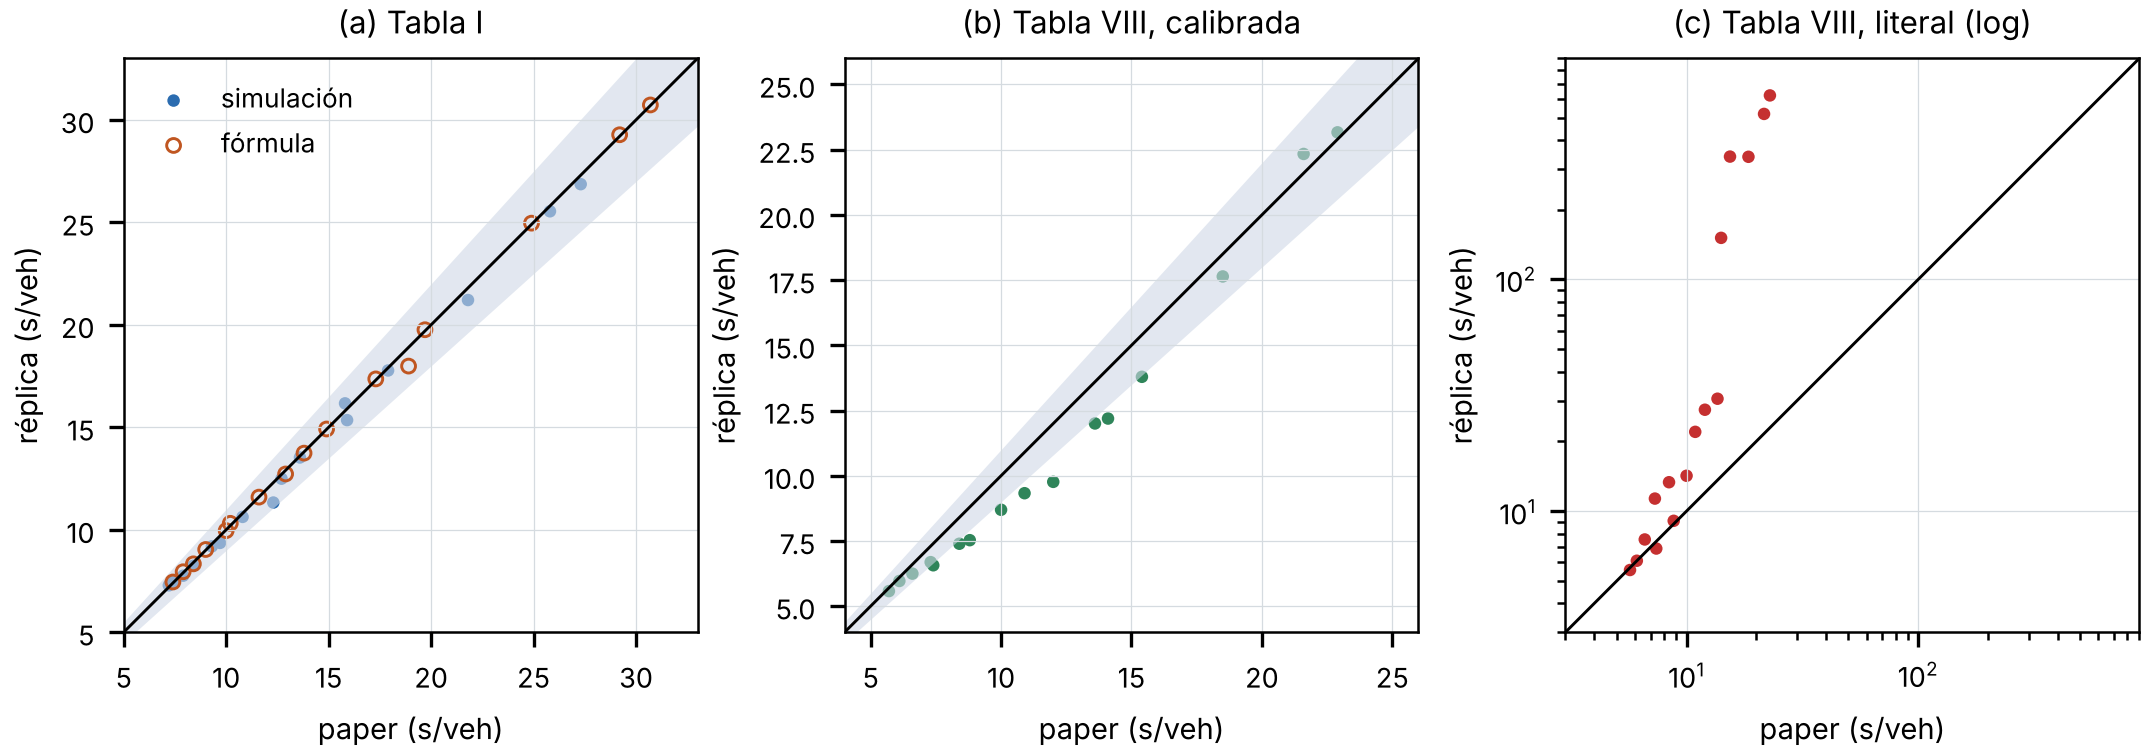
\includegraphics[width=\textwidth]{fig_dispersion.png}
\caption{Réplica frente al artículo original (la diagonal es la coincidencia exacta; la banda es $\pm 10$\,\%): (a) Tabla~I del original; (b) Tabla~VIII del original con la lectura calibrada; (c) Tabla~VIII del original con la lectura literal, en escala logarítmica.}
\end{figure}

\begin{figure}[!h]
\centering
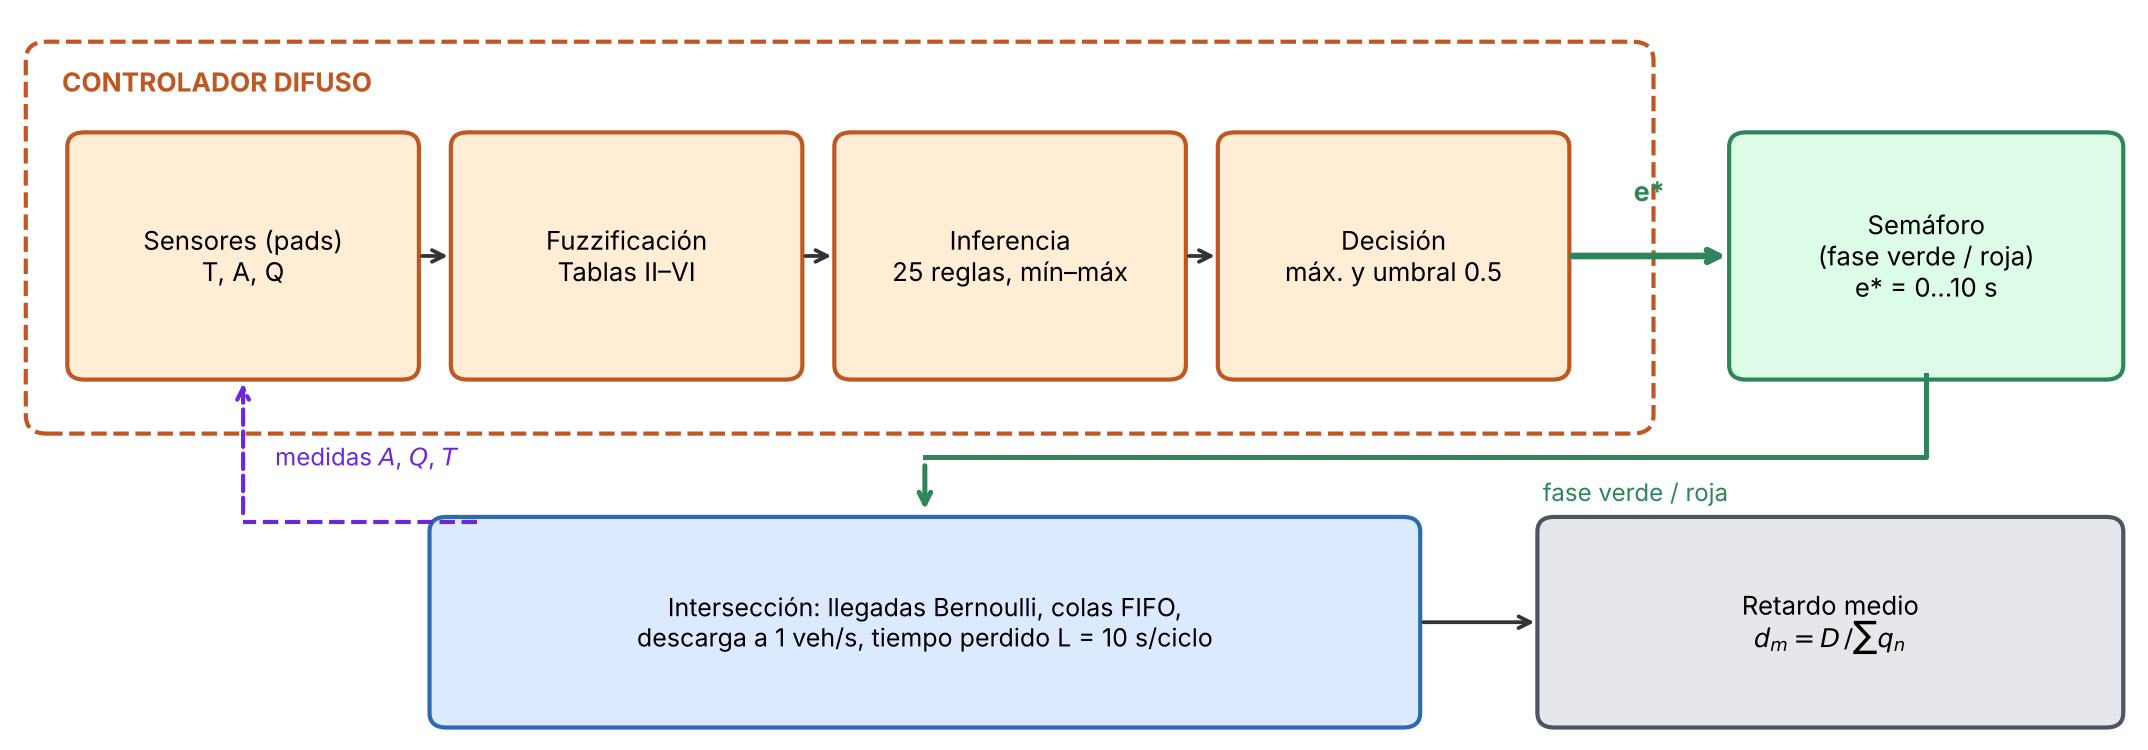
\includegraphics[width=\textwidth]{fig_bloques.png}
\caption{Diagrama de bloques del sistema de control de Pappis y Mamdani (elaboración propia a partir del artículo original).}
\end{figure}

\clearpage
\section{Tablas adicionales}

\begin{table*}[!t]
\caption{Verificación numérica de las deducciones de la Sección~\ref{sec:formulas}: cada fórmula se compara con un cálculo independiente.}
\label{tab:verificacion}
\centering
\footnotesize
\setlength{\tabcolsep}{3pt}
\begin{tabular}{@{}p{0.2\textwidth}p{0.34\textwidth}p{0.17\textwidth}p{0.2\textwidth}@{}}
\toprule
Fórmula & Cálculo independiente con que se compara & Casos & Resultado \\
\midrule
\eqref{eq:retardoR}, \eqref{eq:retardoG}: $D=\sum_n$ colas & suma de las esperas individuales de cada vehículo (cola FIFO con vehículos explícitos) & 1000 escenarios aleatorios & diferencia máxima 0 s$\cdot$veh \\
Término uniforme de \eqref{eq:retardo-webster} & área de la cola de un modelo fluido determinista (paso de 1\,ms) & 5 ciclos $(C,\lambda,q)$ & error relativo máximo 0.013\,\% \\
Término aleatorio de \eqref{eq:retardo-webster} & cola M/D/1 simulada con la recursión de Lindley ($1.5\cdot10^{6}$ clientes) & $X=0.3,\ 0.6,\ 0.8$ & error relativo máximo 0.9\,\% (ruido de la simulación) \\
Reparto $g_i=(y_i/Y)(C_0-L)$ de \eqref{eq:webster} & igualdad de los grados de saturación $X_1=X_2$ & 4 pares de caudales & diferencia máxima $<10^{-15}$ \\
Ciclo $C_0$ de \eqref{eq:webster} & mínimo numérico del retardo de Webster completo, con el mismo reparto de verdes & 4 pares de caudales & el retardo en $C_0$ excede al mínimo en 4.0\,\% como máximo \\
\eqref{eq:lt}, \eqref{eq:mt}: $\max=1-\mu_A$ y $\min=0$ & valores de $\mu_A$ de las Tablas~III y~IV con $x\neq x_0$ & 234 puntos de 12 conjuntos & 0 fallos \\
Regla composicional con entrada exacta & $\max_x\min\{R(x,y),A(x)\}$ frente a la fila $R(x_0,y)$ & 200 relaciones aleatorias & diferencia máxima 0 \\
Conteos & $5\cdot6\cdot6$; $5\cdot5$; $7+5\cdot10$ & 3 conteos & 180; 25; 57 \\
\bottomrule
\end{tabular}
\fuente{\texttt{verificar\_formulas.py} (\texttt{resultados/verificacion\_formulas.json}); los casos aleatorios usan la semilla 2026. La comparación $C_0$ frente al mínimo numérico usa los caudales de la Tabla~VIII (360/360, 720/1080, 1080/1440 y 1440/1440).}
\end{table*}


\begin{table}[!t]
\caption{Efecto de borde del horizonte: aumento relativo del retardo medio al sumar la espera residual de los vehículos que siguen en cola en $t=H$ (20 réplicas de 7200\,s, 16 flujos).}
\label{tab:borde}
\centering
\footnotesize
\begin{tabular}{@{}lrr@{}}
\toprule
Controlador & Media (\%) & Máximo (\%) \\
\midrule
Ciclo fijo & 0.28 & 0.87 \\
Difuso, lectura calibrada & 0.17 & 0.33 \\
Difuso, lectura literal (saturada) & 8.1 & 51.8 \\
\bottomrule
\end{tabular}
\fuente{simulaciones propias (\texttt{efecto\_borde.py}) con las mismas llegadas, con y sin \texttt{Sim.residual\_delay}.}
\end{table}


\end{document}
